\documentclass[11pt,a4paper]{article}
\usepackage[margin=1in]{geometry}
\usepackage[utf8]{inputenc}
\usepackage[T1]{fontenc}
\usepackage{mathptmx}
\usepackage{amsmath}
\usepackage{amssymb}
\usepackage{graphicx}
\usepackage{booktabs}
\usepackage{parskip}
\usepackage{hyperref}
\usepackage{natbib}
\usepackage{caption}
\captionsetup{font=small, labelfont=bf, justification=justified, singlelinecheck=false}

% Supplementary figure/table/section numbering: S1, S2, ...
\renewcommand{\thefigure}{S\arabic{figure}}
\renewcommand{\thetable}{S\arabic{table}}
\renewcommand{\thesection}{S\arabic{section}}
\renewcommand{\thesubsection}{S\arabic{section}.\arabic{subsection}}

\title{\textbf{Supplementary Materials}\\[6pt]
\large Thinking With Models Through Simulation}
\author{Kenny Yu\\KU Leuven \& University of Hasselt\\\texttt{kenny.yu@kuleuven.be}}
\date{}

\begin{document}
\maketitle


% ============================================================
% Section S1: DDM Transfer Demonstration
% ============================================================

\section{Transfer Demonstration: Applying the Simulation Thinking Cycle to a Stochastic Decision Model}
\label{sec:s1}

\subsection*{Purpose}

The main text develops the Simulation Thinking Cycle using two deterministic, low-dimensional associative learning models. That choice was deliberate: deterministic models produce a single trajectory per parameter setting, which makes each diagnostic step easy to trace by hand. The cycle's logic, however, does not depend on determinism or low dimensionality. This section provides a transfer demonstration using a qualitatively different model class, the drift diffusion model (DDM; \citealt{ratcliff1978theory, ratcliff2008diffusion}), to show that the same diagnostic practices apply while the implementation details change. The following subsections walk through all six steps of the Simulation Thinking Cycle explicitly, then examine a structural mimicry result in detail. Supplementary Figures~S1--S3 accompany this demonstration; Figures~S2 and~S3 extend aspects of the accuracy-equivalence result not visualized in the main text (companion code: \texttt{analysis/S1\_ddm\_demonstration.R}). The goal is not to represent the full inferential workflow used in contemporary DDM applications---parameter estimation, model fitting, or complexity-penalized adjudication---but to show that the cycle's diagnostic logic extends when predictions become stochastic and distributional.

\subsection*{The Model}

The DDM models a two-choice decision as a noisy accumulation process. A decision variable $x(t)$ starts at the midpoint $a/2$ and evolves as
\[
  x(t + \Delta t) \;=\; x(t) + v\,\Delta t + \sqrt{\Delta t}\,\varepsilon_t,
\]
where $v$ is the drift rate (net evidence for the correct option), $a$ is boundary separation (caution), and $\varepsilon_t \sim \mathcal{N}(0, 1)$ is momentary noise with diffusion coefficient $s = 1$. The process terminates when $x$ first reaches the upper boundary $a$ (correct response) or the lower boundary $0$ (error). Total response time is decision time plus a non-decision component $t_0$ representing encoding and motor execution. Simulations use the Euler-Maruyama approximation with $\Delta t = 0.001$\,s and a maximum decision time of $6.0$\,s.

\subsection*{Applying the Simulation Thinking Cycle}

\textbf{Question.} Three questions motivate this demonstration. (1)~What determines choice accuracy in the DDM? (2)~Can two parameter configurations be indistinguishable to a researcher who measures only accuracy? (3)~What observation function would resolve that indistinguishability?

\textbf{Formalize.} Writing the DDM as a stochastic differential equation produces an immediate analytical result. For the symmetric DDM with diffusion coefficient $s = 1$ and starting point $x_0 = a/2$, the probability of a correct response equals
\[
  P(\text{correct}) \;=\; \frac{1}{1 + e^{-va}}.
\]
This formula follows from applying the optional stopping theorem to the exponential martingale $e^{-2vx/s^2}$; the derivation is standard but not obvious from a verbal description of ``noisy accumulation towards a boundary.'' The key implication is that accuracy depends only on the product $va$, not on $v$ and $a$ individually. In this example, formalization yields an analytical constraint before simulation is run, which is itself a teaching point: formalization can reveal structural properties that verbal descriptions leave implicit. Simulation remains necessary, however, to determine the size and shape of the RT differences---and to show how the choice of observation function governs apparent indistinguishability. The two steps are complementary rather than substitutes: formalization narrows the space of possible outcomes; simulation populates that space with magnitudes, shapes, and sensitivities that equations alone do not specify.

\textbf{Anticipate.} Three predictions follow. First, accuracy: any two configurations sharing the same $va$ product will produce identical theoretical accuracy. Configs~A ($v = 0.30$, $a = 2.0$) and B ($v = 0.60$, $a = 1.0$) both have $va = 0.60$, so both should produce $P(\text{correct}) = 1/(1 + e^{-0.6}) \approx 64.6\%$. This prediction is a mathematical certainty conditional on the formalization, not a probabilistic conjecture. Second, RT location: Config~A has slow drift and a wide boundary, requiring more time to reach the criterion, so mean RT should be substantially higher than for Config~B. Third, RT shape: both distributions should be right-skewed, with Config~A showing greater spread.

\textbf{Simulate.} Monte Carlo simulation: 2000 independent trials per configuration, each drawing fresh noise at every time step, with \texttt{set.seed(2026)} for reproducibility. The output is a data frame of (RT, response) pairs per configuration. Implementation choices include the replication count (2000 trials), the time step ($\Delta t = 0.001$\,s), the maximum decision time ($6.0$\,s), and the Euler-Maruyama discretization. Varying the replication count would affect the precision of summary statistics but not their qualitative values; varying $\Delta t$ introduces discretization bias that can be made negligible by choosing $\Delta t$ small relative to the decision timescale.

\textbf{Surprise.} Simulation confirms all three predictions. Accuracy: 65.2\% for Config~A and 65.8\% for Config~B, both within Monte Carlo variability of the theoretical 64.6\%. The confirmation is not surprising given the analytical derivation, but serves as a numerical check that the simulation is correctly implemented. Mean correct RT: 1.20\,s vs.\ 0.45\,s, a factor of approximately 2.7 -- the magnitude of this difference is the genuine empirical content of the simulation. RT standard deviation: 0.59\,s vs.\ 0.21\,s. Mean error RT: 1.12\,s vs.\ 0.45\,s. All RT-based summary statistics diverge while accuracy does not.

\textbf{Reflect.} The accuracy equivalence is a structural property of the present symmetric fixed-boundary DDM, not a coincidence of parameterization. No within-model parameter adjustment can distinguish configurations with equal $va$ when accuracy is the observation function, because the formula $P(\text{correct}) = \text{sigmoid}(va)$ is invariant to the individual values of $v$ and $a$ while their product is fixed. The RT distribution difference is also structural within the present formulation in the sense that holding $va$ constant does not preserve RT distributions when $v$ and $a$ vary separately. The observation function therefore determines which theoretical distinctions survive into data. This is an instance of the observation-function principle from Section~2.3 of the main text.

\subsection*{A Structural Mimicry Result}

\emph{Question.} Consider two parameter configurations, both starting with no prior information ($x_0 = a/2$):

\begin{center}
\begin{tabular}{lcccc}
\toprule
 & $v$ & $a$ & $t_0$ & $v \times a$ \\
\midrule
Config~A (slow drift, wide boundary) & 0.30 & 2.0 & 0.20 & 0.60 \\
Config~B (fast drift, narrow boundary) & 0.60 & 1.0 & 0.20 & 0.60 \\
\bottomrule
\end{tabular}
\end{center}

\emph{Prediction checkpoint.} Before simulating, commit to a prediction: will these two configurations produce the same or different behavior?

\emph{Simulate and Surprise.} Accuracy follows $P(\text{correct}) = 1/(1 + e^{-va})$, which depends only on the product $v \times a$. Because both configurations share $v \times a = 0.60$, they produce identical theoretical accuracy ($1/(1 + e^{-0.6}) \approx 64.6\%$), confirmed by simulation (Config~A: 65.2\%; Config~B: 65.8\%). A researcher measuring only choice accuracy cannot distinguish the configurations.

This is a \emph{structural} result within the symmetric fixed-boundary DDM, not a coincidence of parameterization. For this model, accuracy is invariant to all $(v, a)$ pairs with the same product. No within-model parameter adjustment can break this equivalence as long as the product is held constant; it follows from the model's equations.

\emph{Structural vs.\ parametric, and the observation function.} The equivalence is strict only under one observation function. Figure~S1 shows full RT distributions for both configurations. Despite identical accuracy, the distributions differ markedly: Config~A produces wider, slower distributions; Config~B produces narrower, faster distributions. Mean correct RT differs by a factor of approximately 2.7 (Table~S1). Figure~S2 presents the same four summary statistics as a bar chart, making the contrast between identical accuracy and divergent RT-based metrics immediately visible. A researcher who records only accuracy will observe perfect mimicry; a researcher who records response time will not.

This is exactly the observation-function principle from Section~2.3 of the main text: the mapping from latent state to observable determines which theoretical distinctions survive into behavior.

\begin{table}[htbp]
\centering
\small
\caption{Summary statistics for the two DDM configurations. Both have theoretical accuracy $\approx 64.6\%$; all RT-based metrics diverge substantially. (Simulated, $N = 2000$ trials per configuration, \texttt{set.seed(2026)}.)}
\label{tab:s1_stats}
\begin{tabular}{lcccc}
\toprule
 & Accuracy & Mean RT, correct (s) & RT SD, correct (s) & Mean RT, error (s) \\
\midrule
Config~A & 0.652 & 1.20 & 0.59 & 1.12 \\
Config~B & 0.658 & 0.45 & 0.21 & 0.45 \\
\midrule
Theoretical & 0.646 & -- & -- & -- \\
\bottomrule
\end{tabular}
\end{table}

\begin{figure}[htbp]
\centering
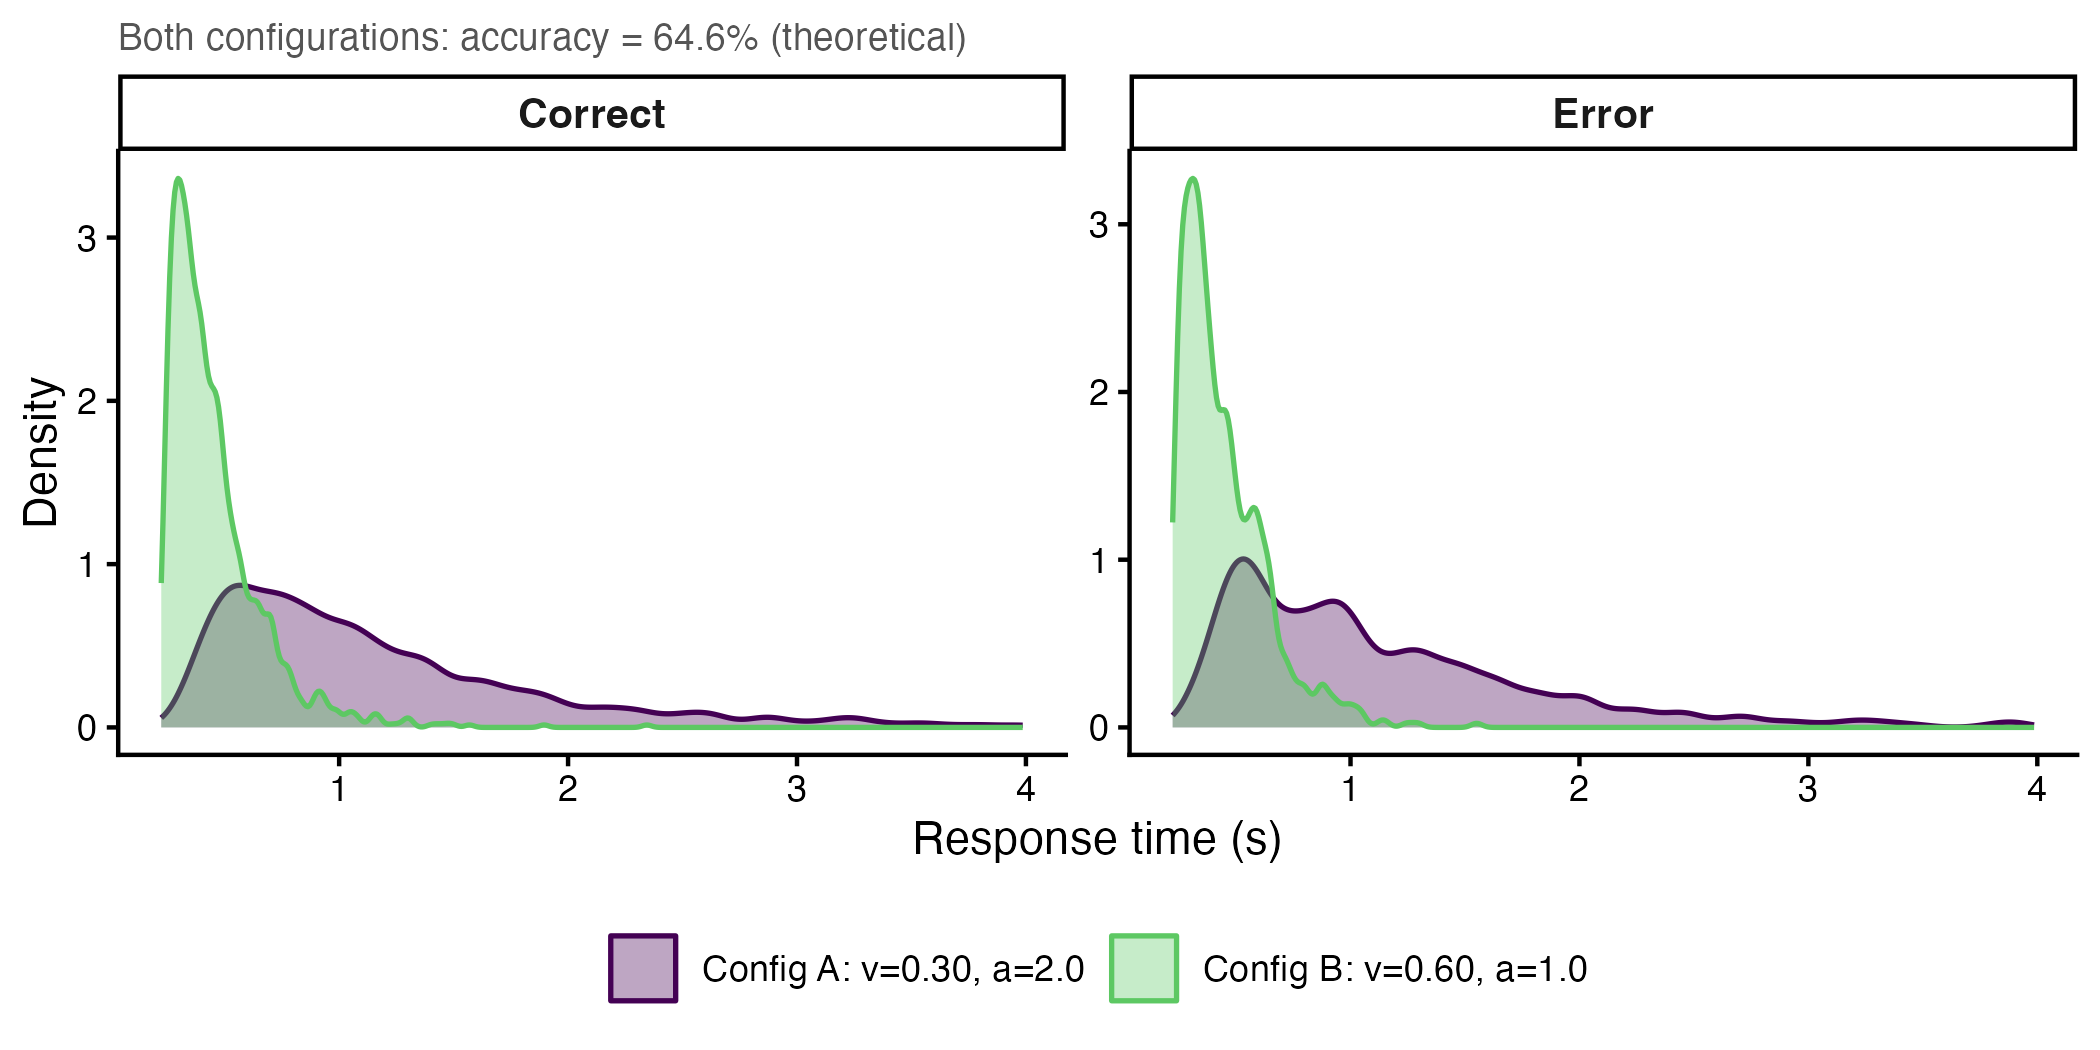
\includegraphics[width=0.85\linewidth]{Figures/figS1_ddm_rt_distributions.pdf}
\caption{RT distributions for the two DDM configurations, separated by correct and error responses. Both configurations share $v \times a = 0.60$ and produce nearly identical accuracy, but the full RT distributions differ markedly in location, spread, and shape. This illustrates the observation-function principle from Section~2.3 of the main text: accuracy alone produces mimicry; the full RT distribution resolves it. ($N = 2000$ trials per configuration.)}
\label{fig:s1_rt}
\end{figure}

\begin{figure}[htbp]
\centering
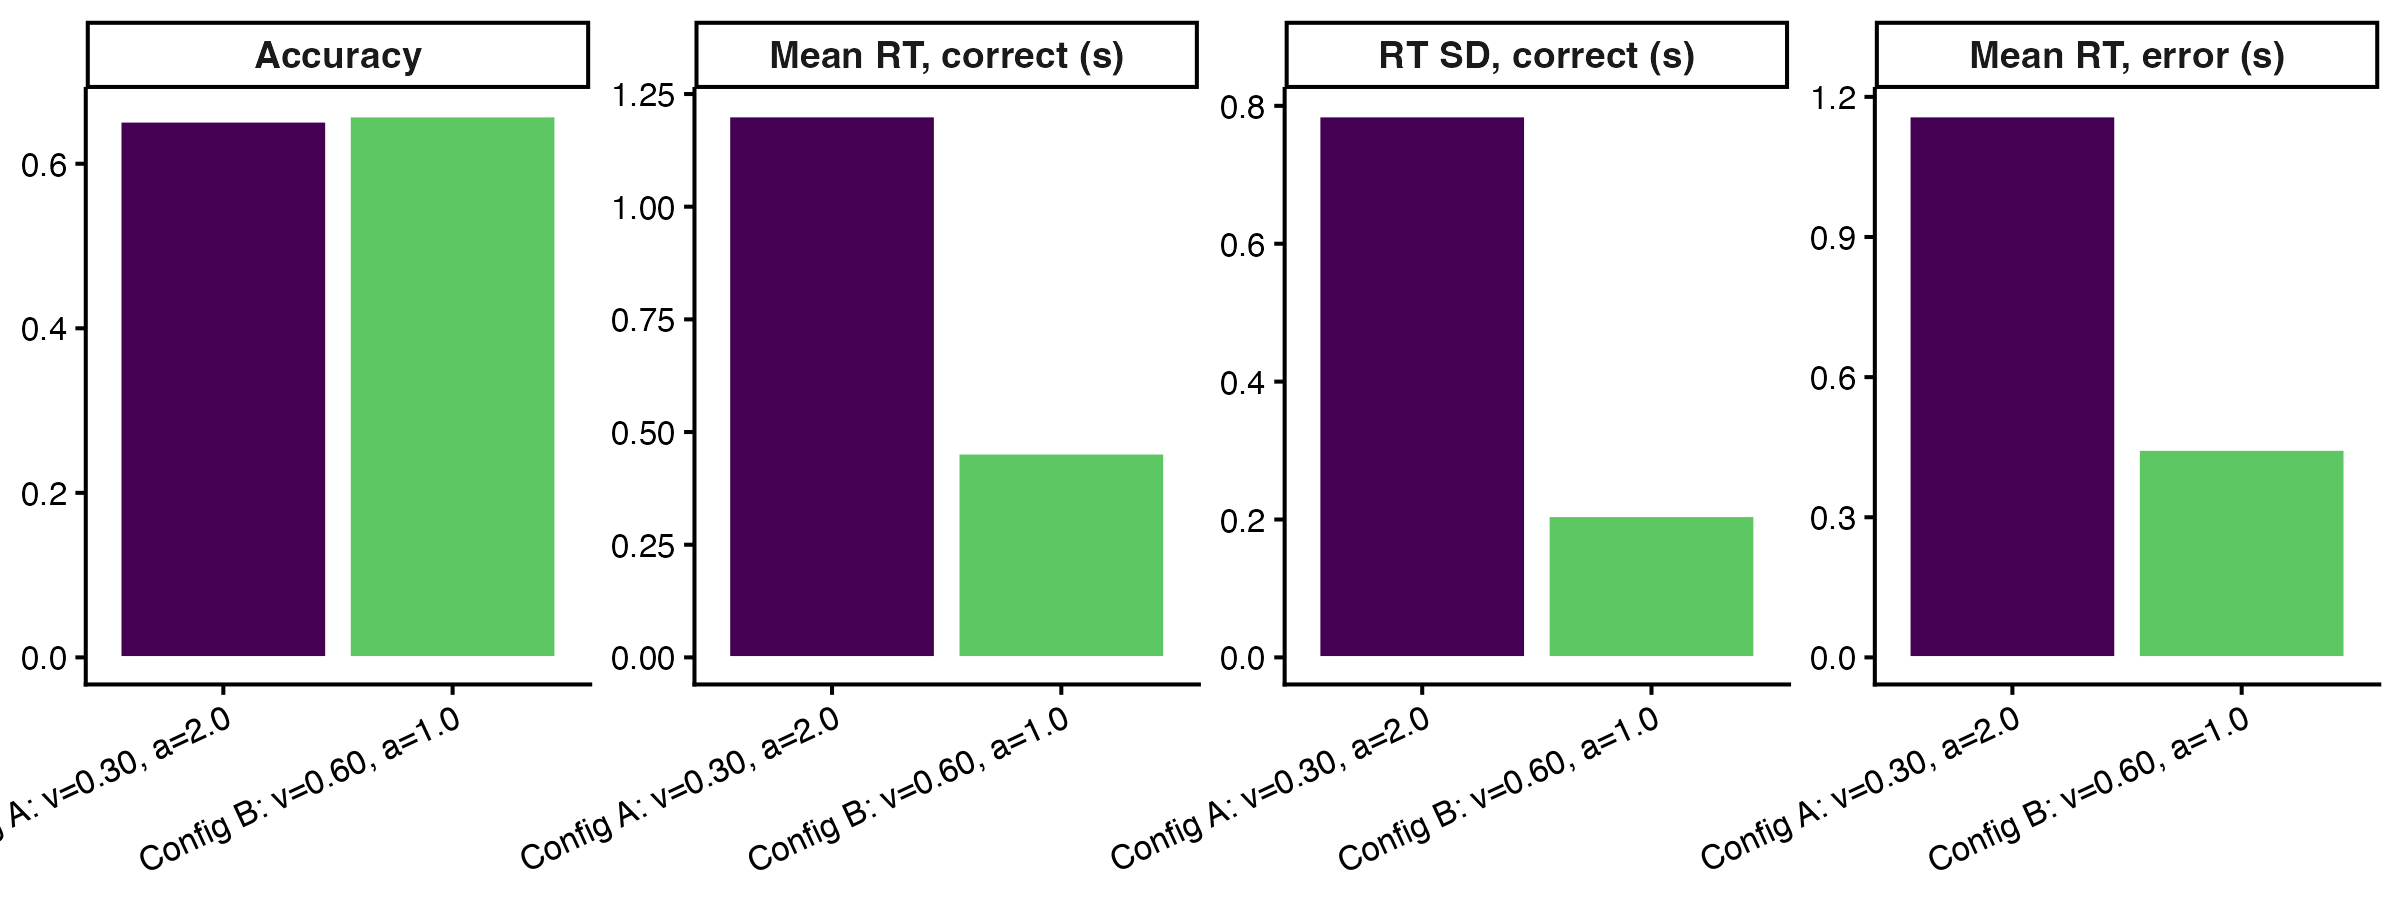
\includegraphics[width=0.90\linewidth]{Figures/figS2_ddm_summary_stats.pdf}
\caption{Summary statistics for both DDM configurations displayed as a bar chart (four panels corresponding to the columns of Table~S1). The near-identical accuracy bars (leftmost panel) contrast with the large differences across the three RT-based metrics. A researcher recording only accuracy (left panel) cannot distinguish the configurations; a researcher recording any RT-based measure can.}
\label{fig:s2_summary}
\end{figure}

\subsection*{The Accuracy Surface: A Structural Property Across the Parameter Space}

Figure~S3 extends the accuracy-equivalence result to the full $(v, a)$ parameter space. The colour encodes $P(\text{correct}) = 1/(1 + e^{-va})$, and white contour lines mark iso-accuracy levels. The dashed white curve traces the hyperbola $v \times a = 0.60$; Configs~A and B both lie on this curve.

Three features of the figure are worth noting. First, iso-accuracy contours are hyperbolas, not ellipses. Moving along any single hyperbola changes $v$ and $a$ in compensating ways while leaving accuracy invariant. Second, there are infinitely many $(v, a)$ pairs on the $va = 0.60$ hyperbola; Configs~A and B are two representatives drawn for pedagogical contrast. Third, the figure reveals the extent to which accuracy collapses the parameter space: a researcher who knows only that $va = 0.60$ cannot reconstruct the individual values of $v$ and $a$, though they could reconstruct the mean RT, which depends on $v$ and $a$ separately rather than on their product alone. Accuracy alone is therefore insufficient to identify $v$ and $a$ separately---it maps the two-dimensional $(v, a)$ space onto a one-dimensional product.

\begin{figure}[htbp]
\centering
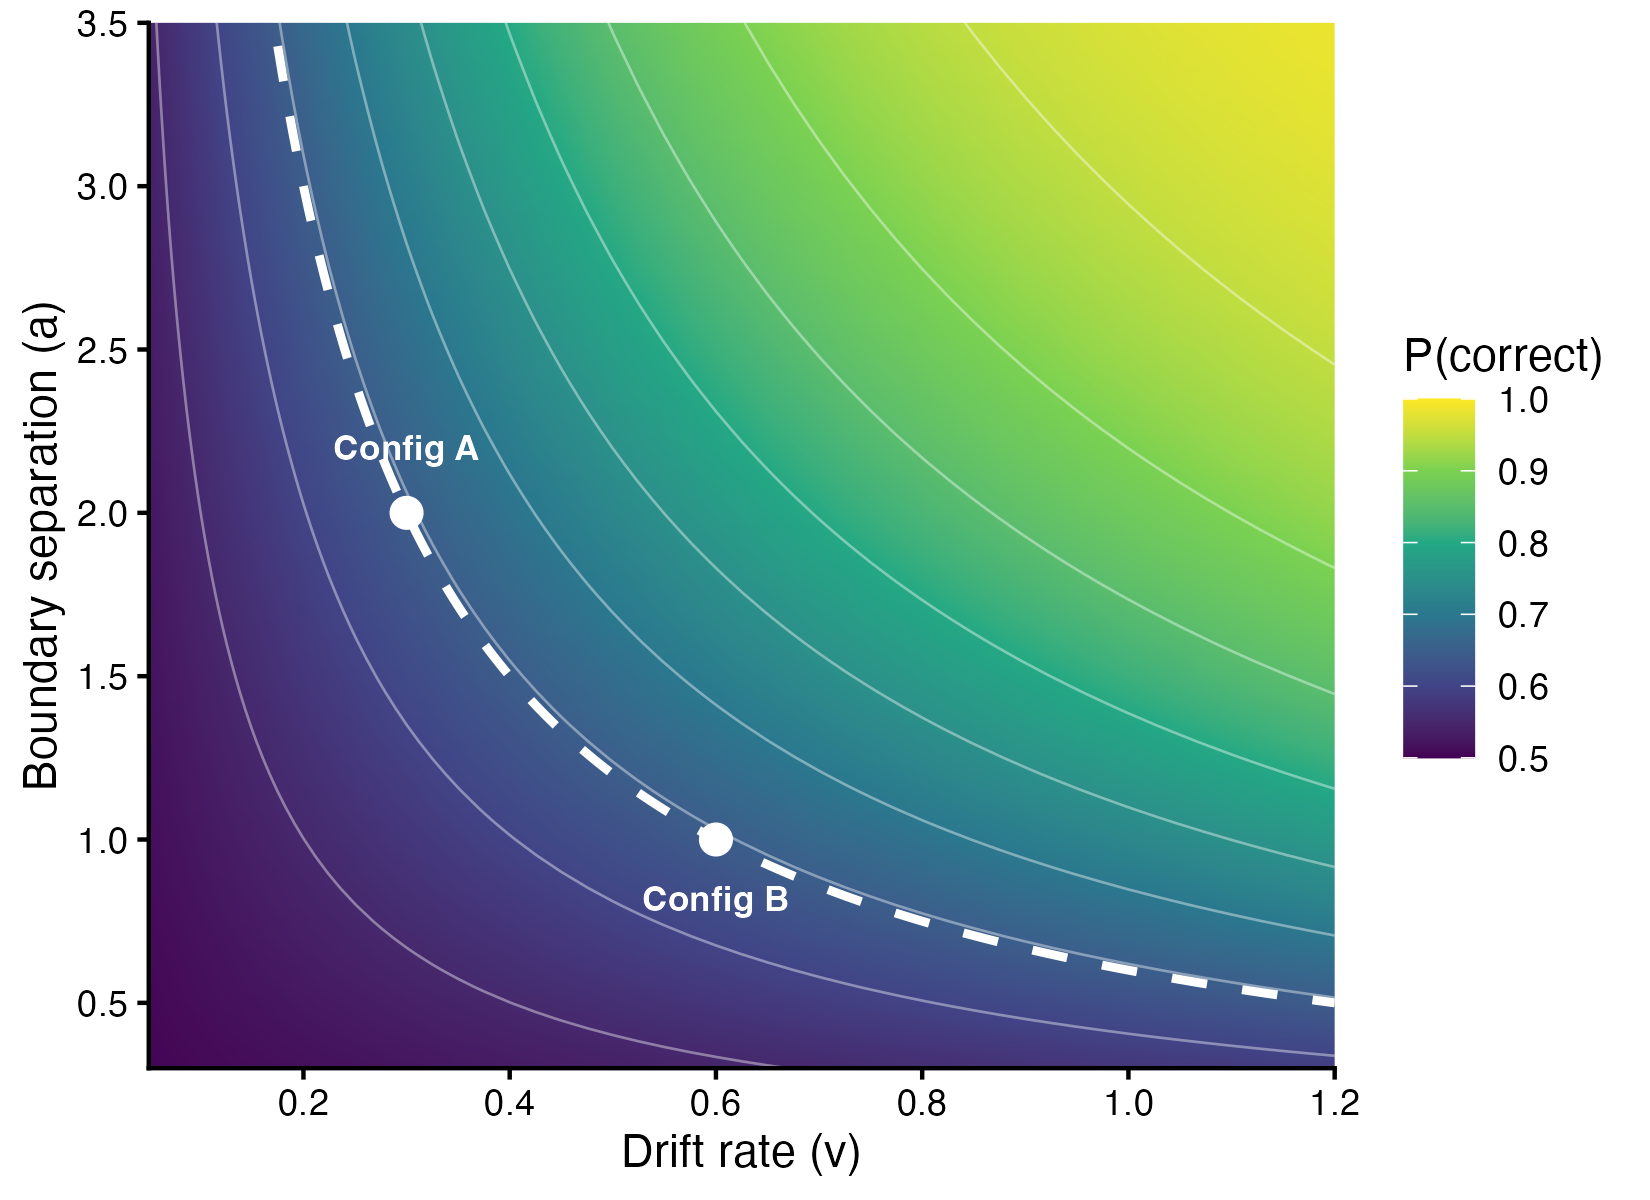
\includegraphics[width=0.78\linewidth]{Figures/figS3_ddm_accuracy_surface.pdf}
\caption{Accuracy surface $P(\text{correct}) = 1/(1 + e^{-va})$ over the $(v, a)$ parameter space. White contours mark iso-accuracy levels; the dashed white curve traces the $v \times a = 0.60$ hyperbola on which Config~A ($v = 0.30$, $a = 2.0$) and Config~B ($v = 0.60$, $a = 1.0$) both lie. Any two points on the same contour are indistinguishable by accuracy alone. The RT distribution -- which depends on $v$ and $a$ individually, not only their product -- resolves the ambiguity.}
\label{fig:s3_surface}
\end{figure}

\subsection*{What Changes and What Stays the Same}

Applying the Simulation Thinking Cycle to the DDM requires adapting each step, but the diagnostic logic at each step is unchanged.

\textbf{Anticipate.} The anticipation is no longer a single scalar but a distributional prediction: what shape, location, and spread should the RT distribution have? The prediction checkpoint becomes a commitment about a distribution, not a trajectory. Stating distributional predictions before simulating exposes commitments that scalar predictions can obscure; for example, committing to a specific shape (Wald-like, heavily right-skewed) before running the simulation makes it possible to notice if the simulation produces a different shape.

\textbf{Simulate.} A single deterministic run no longer suffices. The Simulate step becomes a Monte Carlo procedure: run many replications, each with fresh noise draws, and characterize the resulting distribution. The DDM example used 2000 trials per configuration; models with more parameters or slower dynamics may require substantially more. The convergence of summary statistics as a function of replication count is itself diagnostic: instability in mean RT across runs of 500, 1000, and 2000 trials would warrant a higher replication count before drawing conclusions.

\textbf{Surprise.} The Surprise step now compares a predicted distribution against an obtained distribution, rather than two scalar values. The mimicry example illustrates why scalar comparisons alone can mislead: accuracy is near-identical, while mean RT differs by a factor of 2.7, and the full distributions (Figure~S1) reveal additional shape differences. Examining multiple summary statistics -- and especially the full distribution -- is necessary for a complete Surprise step in stochastic models.

\textbf{Observation function.} The observation function question becomes more consequential in stochastic models, because many summary statistics can be derived from the same underlying process: accuracy, mean RT, RT variance, quantile functions, error RT. Each is a different observation function applied to the same latent dynamics. The commitment anatomy of the observation function is therefore richer: the researcher must declare not only the functional form but also which summary statistic constitutes the dependent variable.

\textbf{Structural vs.\ parametric.} The structural/parametric distinction applies directly. The accuracy equivalence for matched $va$ is structural within the present DDM formulation: it holds across the full $(v,a)$ parameter space conditional on the symmetric-start, flat-boundary, fixed-diffusion-coefficient assumptions, as Figure~S3 makes visible. The RT distribution difference is also structural within the present formulation in the sense that holding $va$ constant does not preserve RT distributions when $v$ and $a$ vary separately. Robustness sweeps over the product $va$ would reveal the accuracy surface; sweeps over individual parameters would reveal the RT surface.

\textbf{Commitment anatomy.} The DDM commitment anatomy can be decomposed analogously to the commitment table in the main text. The \emph{core claim} is noisy evidence accumulation to absorbing boundaries. \emph{Auxiliary assumptions} include: the symmetric starting point ($x_0 = a/2$); Gaussian momentary noise; flat (non-collapsing) boundaries; the additive non-decision time $t_0$. \emph{Implementation choices} include specific values of $v$, $a$, $t_0$; the time step $\Delta t = 0.001$\,s; the maximum decision time $6.0$\,s; and the Euler-Maruyama discretization. Each auxiliary could be changed independently to test whether a predicted pattern survives. Replacing the flat boundary with a collapsing boundary is an auxiliary change that would alter the RT distribution shape without affecting the core accumulation claim; it would also break the $P(\text{correct}) = \text{sigmoid}(va)$ result, which depends on the flat-boundary assumption.

\subsection*{What the Demonstration Does Not Show}

This section demonstrates transferability of the cycle's logic, not of the specific techniques. Three complications that arise in real DDM applications but are not illustrated here are: (1)~\emph{between-trial parameter variability}, which the full Ratcliff diffusion model includes and which changes the predicted RT distribution shape, particularly producing the heavy-tailed error RT distributions observed empirically; (2)~\emph{model fitting}, which in the DDM requires maximum likelihood or Bayesian methods applied to the full RT distribution, not simple moment-matching; and (3)~\emph{model comparison under complexity}, where DDM variants differ in the number of variability parameters and complexity penalties matter for adjudication. All three belong to the post-data phase; the present demonstration shows only the pre-data reasoning structure.

A fourth limitation concerns the relationship between the pre-data and post-data phases. Confirming what the model commits to -- and visualizing those commitments across the parameter space -- does not establish that the DDM is correct as a model of human decision-making, nor that the parameter values $(v, a, t_0)$ can be recovered from a finite sample of noisy RTs. The model recovery question -- whether a researcher who observes data generated by one parameter configuration can correctly identify the generating parameters -- requires data-level fitting and is a separate analysis. Section~S3 of these materials illustrates this logic for the associative learning models.

\clearpage


% ============================================================
% Section S2: Robustness Analysis
% ============================================================

\section{Robustness Analysis: Quantitative Detail}
\label{sec:s2}

Section~4.7 of the main text reports four robustness checks on the critical-test divergence between Rescorla-Wagner and Mackintosh. This section provides complete numerical results for each check, supplementing the visual summaries in Figures~12--14 of the main text (companion code: \texttt{analysis/07\_robustness.R}).

\subsection{Design and Parameter Convention}
\label{sec:s2_design}

All four checks use a three-phase blocking design: Phase~1 (20 trials, A+), Phase~2 (20 trials, AB+), Phase~3 (20 trials, B+). The reference parameters are $\alpha_A = 0.4$, $\beta = 0.3$ for Rescorla-Wagner, and $S = \beta = 0.3$, $\beta_{\text{up}} = 0.03$, $\beta_{\text{down}} = 0.15$, $\alpha_0 = 0.5$ for Mackintosh. Mackintosh's salience parameter $S$ is yoked to RW's $\beta$ throughout, following the fair-comparison rationale in Section~3.1 of the main text.

The checks use 20 trials per phase rather than the 10 trials used in the main tutorial demonstrations. The longer training amplifies divergence between the models and makes qualitative patterns in the robustness figures clearer. The same qualitative patterns were confirmed under the main text's 10-trial-per-phase design via spot checks in the companion code (\texttt{analysis/07\_robustness.R}).

At the Phase~2/Phase~3 boundary under the reference parameters, $V_B$ differs markedly between the two models before any reset: $V_B(\text{RW}) = 0.039$ and $V_B(\text{Mack}) = 0.634$. This difference reflects a fundamental architectural distinction. In Rescorla-Wagner, global prediction error keeps $V_B$ low during Phase~2 because $V_A$ is already high after Phase~1 training, leaving little prediction error for B to acquire. In Mackintosh, the local error term $(\lambda - V_B)$ remains large throughout Phase~2 because $V_B$ starts near zero, allowing $V_B$ to accumulate despite the suppressed attention to B. Resetting $V_B$ to zero at the Phase~3 boundary removes this carry-over and places both models on equal footing; the generalization sweep in Section~\ref{sec:s2b} asks what happens when the carry-over is only partially removed.

\subsection{Check A: Observation Function Sensitivity}
\label{sec:s2a}

The $\alpha_A \times \beta$ parameter sweep (81 combinations, $\alpha_A, \beta \in \{0.1, 0.2, \ldots, 0.9\}$) was repeated under three observation functions applied to Phase~3 final $V_B$: raw $V_B$ (identity mapping), sigmoid with $\gamma = 5$ and $\theta = 0.5$, and threshold with $\theta = 0.3$.

Table~S2 summarizes the results. Under the raw $V$ and sigmoid metrics, divergence is positive and substantial across most of the swept parameter space, with maximum observed values of 0.197 (raw $V$) and 0.224 (sigmoid). The sigmoid metric produces larger maximum divergence because it amplifies differences near its inflection point, which lies between the two models' $V_B$ values for a large portion of the parameter space. Under the threshold metric ($\theta = 0.3$), qualitative disagreement -- defined as the two models falling on opposite sides of the threshold -- was observed in 0 of 81 parameter combinations (0\%). Both models produce $V_B > 0.3$ after 20 Phase~3 trials across the entire swept space, making the threshold metric uninformative at this criterion.

This result instantiates the limitation of threshold observation functions noted in Box~2 of the main text. When both models' outputs fall on the same side of the criterion, threshold-based comparisons cannot detect divergence regardless of its magnitude. Moving the threshold to $\theta = 0.85$, near the midpoint between the two models' $V_B$ values at the reference parameters (RW = 0.922, Mack = 0.766), would produce qualitative disagreement at some parameter combinations, but would still miss divergence at settings where both models fall above or below 0.85. The continuous-valued metrics -- raw $V$ and sigmoid -- do not have this problem.

\begin{table}[htbp]
\centering
\small
\caption{Observation function sensitivity. The parameter sweep covers 81 combinations of $\alpha_A \in [0.1, 0.9]$ and $\beta \in [0.1, 0.9]$ (step 0.1). At the reference parameters ($\alpha_A = 0.4$, $\beta = 0.3$): $V_B(\text{RW}) = 0.922$, $V_B(\text{Mack}) = 0.766$. The sigmoid divergence at reference is $|\sigma(0.922) - \sigma(0.766)|$ with $\sigma(v) = 1/(1 + e^{-5(v-0.5)})$. Visual distribution of divergence across the parameter space is shown in Figure~12 of the main text.}
\label{tab:s2_obs}
\begin{tabular}{llcc}
\toprule
Metric & Parameters & At reference params & Maximum (81 combos) \\
\midrule
Raw $V_B$ & -- & 0.156 & 0.197 \\
Sigmoid & $\gamma = 5,\;\theta = 0.5$ & 0.101 & 0.224 \\
Threshold & $\theta = 0.3$ & 0 & 0 \\
\bottomrule
\end{tabular}
\end{table}

\subsection{Check B: Reset Assumption Sensitivity}
\label{sec:s2b}

The standard condition resets $V_B$ to zero at the Phase~3 boundary (generalization fraction $g = 0$). Check~B varies $g \in \{0, 0.25, 0.50, 0.75, 1.00\}$, setting the Phase~3 starting value to $g \times V_B^{\text{P2}}$, where $V_B^{\text{P2}}$ is the Phase~2 final value for each model. Mackintosh's attention parameter $\alpha_B$ is preserved in all conditions.

Table~S3 shows the results. At $g = 0$, divergence is 0.156 with RW acquiring faster ($V_B = 0.922$) than Mackintosh ($V_B = 0.766$) after 20 Phase~3 trials. As $g$ increases, Mackintosh gains an increasing head start because its Phase~2 carry-over ($V_B^{\text{P2}} = 0.634$) is much larger than RW's ($V_B^{\text{P2}} = 0.039$). The divergence decreases monotonically as $g$ increases: from 0.156 at $g = 0$ to 0.001 at $g = 1.0$, where the ordering effectively disappears and Mackintosh's $V_B$ (0.927) marginally exceeds RW's (0.925).

The interpretation is direct. The critical test discriminates the models because Mackintosh's suppressed attention slows Phase~3 acquisition. The reset removes the carry-over advantage that Mackintosh would otherwise hold from its Phase~2 local-error learning. When carry-over is fully retained ($g = 1.0$), the Phase~2 head start swamps the Phase~3 attention effect and the models converge. Within the present setup, this indicates that the reset assumption is load-bearing: researchers who allow strong generalization from Phase~2 to Phase~3 should expect near-zero or reversed divergence, even when the underlying mechanism difference is real.

\begin{table}[htbp]
\centering
\small
\caption{Reset assumption sensitivity. $V_B$ at Phase~3 start is set to $g \times V_B^{\text{P2}}$, where $V_B^{\text{P2}}(\text{RW}) = 0.039$ and $V_B^{\text{P2}}(\text{Mack}) = 0.634$. Mackintosh attention $\alpha_B$ is preserved in all conditions. Signed divergence is $V_B(\text{RW}) - V_B(\text{Mack})$; positive values indicate RW acquires faster. Reference parameters: $\alpha_A = 0.4$, $\beta = 0.3$. Visual display is in Figure~13 of the main text.}
\label{tab:s3_reset}
\begin{tabular}{ccccc}
\toprule
$g$ & $V_B(\text{RW})$ & $V_B(\text{Mack})$ & Signed divergence & $|$Divergence$|$ \\
\midrule
0.00 & 0.922 & 0.766 & $+$0.156 & 0.156 \\
0.25 & 0.923 & 0.831 & $+$0.092 & 0.092 \\
0.50 & 0.924 & 0.863 & $+$0.061 & 0.061 \\
0.75 & 0.925 & 0.895 & $+$0.030 & 0.030 \\
1.00 & 0.925 & 0.927 & $-$0.001 & 0.001 \\
\bottomrule
\end{tabular}
\end{table}

\subsection{Check C: Divergence Metric Equivalence}
\label{sec:s2c}

Three divergence metrics were evaluated at the reference parameters ($\alpha_A = 0.4$, $\beta = 0.3$) to determine whether the qualitative conclusion depends on which metric is used.

Table~S4 shows the results. The absolute difference between the two models' Phase~3 final $V_B$ is 0.156; the ratio $V_B(\text{Mack})/V_B(\text{RW})$ is 0.831; and the learning rate proxy (slope of $V_B$ over the first five Phase~3 trials, estimated by linear regression) is 0.100/trial for RW and 0.011/trial for Mackintosh, a ratio of 0.111. All three metrics agree qualitatively: RW acquires B faster than Mackintosh in Phase~3. The slope ratio is the most pronounced (0.111), reflecting the initial period when Mackintosh's attention suppression is strongest ($\alpha_B \approx 0.019$ at Phase~3 start) and attention recovery has barely begun.

\begin{table}[htbp]
\centering
\small
\caption{Divergence metric equivalence at reference parameters ($\alpha_A = 0.4$, $\beta = 0.3$). Phase~3 uses 20 trials. $V_B(\text{RW}) = 0.922$, $V_B(\text{Mack}) = 0.766$ at Phase~3 end. The learning rate proxy is the slope of $V_B$ over Phase~3 trials 1--5, estimated by linear regression.}
\label{tab:s4_metric}
\begin{tabular}{lll}
\toprule
Metric & Formula & Value \\
\midrule
Absolute difference & $|V_B(\text{RW}) - V_B(\text{Mack})|$ & 0.156 \\
Ratio & $V_B(\text{Mack}) / V_B(\text{RW})$ & 0.831 \\
RW learning rate proxy & slope$(V_B^{\text{RW}}$, trials 1--5) & 0.100 per trial \\
Mack learning rate proxy & slope$(V_B^{\text{Mack}}$, trials 1--5) & 0.011 per trial \\
Slope ratio (Mack/RW) & -- & 0.111 \\
\bottomrule
\end{tabular}
\end{table}

\subsection{Check D: Attention Parameter Sensitivity}
\label{sec:s2d}

The Mackintosh model's attention parameters ($\beta_{\text{up}}$, $\beta_{\text{down}}$) were varied over a $4 \times 4$ grid: $\beta_{\text{up}} \in \{0.01, 0.03, 0.05, 0.10\}$ and $\beta_{\text{down}} \in \{0.05, 0.10, 0.15, 0.30\}$. All other parameters were held at reference values. Because RW has no attention parameters, $V_B(\text{RW}) = 0.922$ is constant across all 16 combinations. Results are shown in Table~S5 and Figure~14 of the main text.

Three patterns emerge from the table.

First, $\alpha_B$ at the Phase~2/Phase~3 boundary depends only on $\beta_{\text{down}}$, not on $\beta_{\text{up}}$. Within each $\beta_{\text{down}}$ group (each horizontal row block in Table~S5), $\alpha_B$ is constant regardless of $\beta_{\text{up}}$. This is because during Phase~2 (AB+ compound), B is a poorer predictor of the outcome than A (which already has high associative strength), so the attention-increase condition for B is never satisfied. Attention to B can only decrease in Phase~2, making $\beta_{\text{up}}$ irrelevant for the Phase~2 dynamics. The $\beta_{\text{up}}$ parameter becomes relevant only in Phase~3, when B is trained alone and begins to predict the outcome.

Second, the direction of the divergence depends on $\beta_{\text{up}}$, not on $\beta_{\text{down}}$. The five combinations where Mack exceeds RW (negative signed divergence) all have $\beta_{\text{up}} \geq 0.05$. At these values, attention to B recovers rapidly once B is trained alone in Phase~3, accelerating $V_B$ acquisition in Mackintosh to the point where it overtakes RW. The reference parameters ($\beta_{\text{up}} = 0.03$, $\beta_{\text{down}} = 0.15$, marked with $\dagger$ in Table~S5) fall in the RW $>$ Mack regime.

Third, the reversal at high $\beta_{\text{up}}$ is theoretically informative rather than a stability concern. It specifies a precise prediction of Mackintosh's architecture: with fast attention recovery, the blocked cue is reacquired more quickly than a fixed-rate model (RW) predicts. Researchers who expect retarded reacquisition of blocked cues are implicitly assuming slow attention recovery ($\beta_{\text{up}}$ in the lower range of the table). Researchers who expect facilitated reacquisition are implicitly assuming fast recovery. The attention parameter sweep makes this implicit assumption explicit.

The sweep is illustrative rather than exhaustive. The four-point grids for $\beta_{\text{up}}$ and $\beta_{\text{down}}$ were chosen to sample qualitatively distinct regimes---slow and fast attention recovery, slow and fast suppression---rather than to bound the full parameter space or establish distributional claims about Mackintosh's behavior in general. The purpose is to demonstrate how a robustness check over mechanism-specific parameters can reveal the conditional nature of a critical-test prediction: whether RW or Mackintosh predicts faster Phase~3 acquisition is not a fixed theoretical implication but depends on an auxiliary assumption about the speed of attention recovery.

\begin{table}[htbp]
\centering
\small
\caption{Attention parameter sensitivity. Each row shows a $(\beta_{\text{up}},\,\beta_{\text{down}})$ combination with the resulting $\alpha_B$ at the Phase~2/Phase~3 boundary, the Mackintosh final $V_B$ after 20 Phase~3 trials, and the signed divergence $V_B(\text{RW}) - V_B(\text{Mack})$ (positive = RW faster, negative = Mack faster). $V_B(\text{RW}) = 0.922$ in all rows. The reference combination ($\beta_{\text{up}} = 0.03$, $\beta_{\text{down}} = 0.15$) is marked with $\dagger$. Visual display is in Figure~14 of the main text.}
\label{tab:s5_attn}
\begin{tabular}{ccccc}
\toprule
$\beta_{\text{up}}$ & $\beta_{\text{down}}$ & $\alpha_B$ at Phase~3 start & $V_B(\text{Mack})$ & Signed div. \\
\midrule
0.01 & 0.05 & 0.179 & 0.773 & $+$0.150 \\
0.03 & 0.05 & 0.179 & 0.894 & $+$0.029 \\
0.05 & 0.05 & 0.179 & 0.944 & $-$0.021 \\
0.10 & 0.05 & 0.179 & 0.982 & $-$0.060 \\
\midrule
0.01 & 0.10 & 0.061 & 0.554 & $+$0.369 \\
0.03 & 0.10 & 0.061 & 0.807 & $+$0.115 \\
0.05 & 0.10 & 0.061 & 0.905 & $+$0.018 \\
0.10 & 0.10 & 0.061 & 0.974 & $-$0.052 \\
\midrule
0.01 & 0.15 & 0.019 & 0.444 & $+$0.478 \\
$0.03^\dagger$ & $0.15^\dagger$ & 0.019 & 0.766 & $+$0.156 \\
0.05 & 0.15 & 0.019 & 0.887 & $+$0.035 \\
0.10 & 0.15 & 0.019 & 0.970 & $-$0.048 \\
\midrule
0.01 & 0.30 & 0.010 & 0.423 & $+$0.499 \\
0.03 & 0.30 & 0.010 & 0.758 & $+$0.164 \\
0.05 & 0.30 & 0.010 & 0.884 & $+$0.039 \\
0.10 & 0.30 & 0.010 & 0.970 & $-$0.047 \\
\bottomrule
\end{tabular}
\end{table}

\subsection{Summary}
\label{sec:s2_summary}

The four checks collectively establish three points. First, the divergence is robust to continuous-valued observation functions: raw $V$ and sigmoid metrics both show substantial divergence across a wide portion of the sampled parameter space. Threshold-based metrics can miss real divergence entirely when both models' outputs fall on the same side of the criterion. Second, the reset assumption is load-bearing: partial generalization from Phase~2 to Phase~3 progressively reduces the divergence and can reverse the ordering at full generalization, because Mackintosh accumulates much more $V_B$ during Phase~2 via local error learning. Third, the direction of the divergence -- whether RW or Mackintosh acquires B faster in Phase~3 -- depends on $\beta_{\text{up}}$. With slow attention recovery (default $\beta_{\text{up}} = 0.03$), RW acquires faster; with fast recovery ($\beta_{\text{up}} \geq 0.05$), Mackintosh acquires faster. This third finding specifies exactly which empirical outcome a researcher should predict under Mackintosh depending on their assumptions about the attention recovery rate.

\clearpage


% ============================================================
% Section S3: Model Recovery Analysis
% ============================================================

\section{Model Recovery Analysis}
\label{sec:s3}

\subsection{Motivation and Design}
\label{sec:s3_motivation}

Sections~3--4 of the main text ask when RW and Mackintosh produce divergent predictions under idealized conditions. Section~5 asks whether that divergence is statistically detectable given realistic observation noise. This section addresses a further question: if an experimenter ran the critical test and observed a dataset, would a standard fit-based model comparison correctly identify the generating model?

This is the model recovery question \citep{wilson2019ten}. The logic is: generate synthetic data from each candidate model, fit both models to each synthetic dataset, select the better-fitting model, and tabulate how often the generating model is correctly identified. A high recovery rate means the models are distinguishable given the data; a low rate means either the models are too similar, the noise is too large, or the fitting procedure is insensitive. Model recovery is a precondition for designing a worthwhile experiment: if models cannot be recovered from data even in principle, collecting data to adjudicate between them is premature.

\subsection{Methodology}
\label{sec:s3_method}

\textbf{Experimental design.} Three-phase blocking: Phase~1 (20 trials, A+), Phase~2 (20 trials, AB+), Phase~3 (10 trials, B+). Phase~3 is shorter than Phases~1 and~2, reflecting a common experimental constraint. This design produces stronger blocking than the main tutorial demonstration (20 trials per phase vs.\ 10), resulting in greater model separation for recovery.

\textbf{Individual differences and observation noise.} Each simulated participant has an individual learning rate $S_i \sim \text{Beta}(3, 7)$ (mean 0.30, matched to Section~5 of the main text), drawn independently. Additive Gaussian observation noise $\varepsilon_i \sim \mathcal{N}(0, \sigma^2)$ with $\sigma = 1.0$ is applied to each participant's simulated Phase~3 $V_B$ value.

\textbf{Simplified fitting procedure.} This demonstration uses a pedagogically simplified SSE comparison: the mean observed $V_B$ across $N = 30$ participants is compared against each model's prediction at the population mean rate ($\overline{S} = 0.30$). The model with lower sum of squared errors is selected. Under these parameters, the RW model predicts $V_B = 0.722$ and the Mackintosh model predicts $V_B = 0.300$ after Phase~3, a separation of 0.422. A publication-ready analysis would use per-participant maximum likelihood estimation, fit the model to each participant's full response sequence, and apply complexity penalties such as BIC \citep{wilson2019ten, schad2021workflow}. The present approach is an explicit simplification that should be read as a conservative summary-level approximation of recoverability. Strictly, this procedure tests whether the sample mean $V_B$ falls closer to the RW or Mackintosh population prediction; it is a recovery demonstration for a summary-statistic comparison rather than for full trial-level likelihood fitting, and the label ``model recovery'' is used in the pedagogical sense of demonstrating recoverability logic rather than as a claim about the performance of standard fitting algorithms.

\textbf{Replications.} 200 replications per generating model (400 total) with \texttt{set.seed(2026)}.

\subsection{Main Recovery Results}
\label{sec:s3_main}

Table~S6 shows the confusion matrix. The overall recovery rate is 80.8\%. When RW generated the data, the correct model was identified 79.5\% of the time (20.5\% misidentified as Mackintosh). When Mackintosh generated the data, the correct model was identified 82.0\% of the time (18.0\% misidentified as RW).

The modest false-positive rate of approximately 20\% per cell arises primarily from observation noise. When $\sigma = 1.0$ is applied to $V_B$ values in $[0, 1]$, the standard error of the sample mean across $N = 30$ participants is approximately $\sigma/\sqrt{N} = 0.18$. The gap between the two model predictions is 0.422, roughly 2.3 standard error units. This makes the SSE comparison reliable but not certain: some datasets from each generating model will land closer to the other model's prediction by chance. A more sensitive fitting procedure using per-participant information would reduce this error rate.

\begin{table}[htbp]
\centering
\small
\caption{Model recovery confusion matrix. Rows indicate the generating model; columns indicate the model selected by the SSE comparison. Each cell is a percentage of 200 replications. Diagonal entries (bold) are correct recoveries. ($N = 30$, $\sigma = 1.0$, 200 replications per generating model, \texttt{set.seed(2026)}.)}
\label{tab:s6_confusion}
\begin{tabular}{lcc}
\toprule
 & Selected: RW & Selected: Mackintosh \\
\midrule
Generated by RW & \textbf{79.5\%} & 20.5\% \\
Generated by Mackintosh & 18.0\% & \textbf{82.0\%} \\
\bottomrule
\multicolumn{3}{l}{\small Overall recovery rate: 80.8\%}
\end{tabular}
\end{table}

\subsection{Recovery as a Function of Measurement Noise}
\label{sec:s3_noise}

Table~S7 and Figure~S4 show recovery rate as a function of observation noise $\sigma$, holding $N = 30$ fixed. At $\sigma = 0.5$, recovery is 97.5\%, near ceiling. At $\sigma = 1.0$, recovery is 84.0\% (note: this slightly exceeds the main analysis value of 80.8\% due to Monte Carlo variability; both values used independent random draws after the initial seed). At $\sigma = 2.0$ and $\sigma = 3.0$, recovery is 64.5\% and 65.5\%, well below the practical threshold of 80\%. At $\sigma = 5.0$, recovery is 55.0\%, close to chance.

The sharp decline between $\sigma = 1.0$ and $\sigma = 2.0$ has a straightforward explanation. The standard error of the mean $V_B$ across $N = 30$ participants is $\sigma/\sqrt{N}$: approximately 0.18 at $\sigma = 1.0$ and 0.37 at $\sigma = 2.0$. The prediction gap between the two models is 0.422. Expressed in units of the standard error, the gap shrinks from 2.3 (reliable comparison) to 1.1 (unreliable comparison) as $\sigma$ doubles. The SSE comparison behaves like a signal detection problem: the signal is the model prediction gap (0.422), the noise is the sampling variability of the mean, and sensitivity collapses rapidly once noise exceeds roughly half the signal.

\begin{table}[htbp]
\centering
\small
\caption{Recovery rate as a function of observation noise $\sigma$. Each entry is the overall recovery rate (proportion of trials on which the generating model was correctly identified), averaged equally over RW-generating and Mackintosh-generating conditions. 100 replications per generating model per noise level. ($N = 30$; random draws are independent of Table~S6.)}
\label{tab:s7_noise}
\begin{tabular}{cc}
\toprule
Noise ($\sigma$) & Recovery rate \\
\midrule
0.5 & 97.5\% \\
1.0 & 84.0\% \\
2.0 & 64.5\% \\
3.0 & 65.5\% \\
5.0 & 55.0\% \\
\bottomrule
\end{tabular}
\end{table}

\begin{figure}[htbp]
\centering
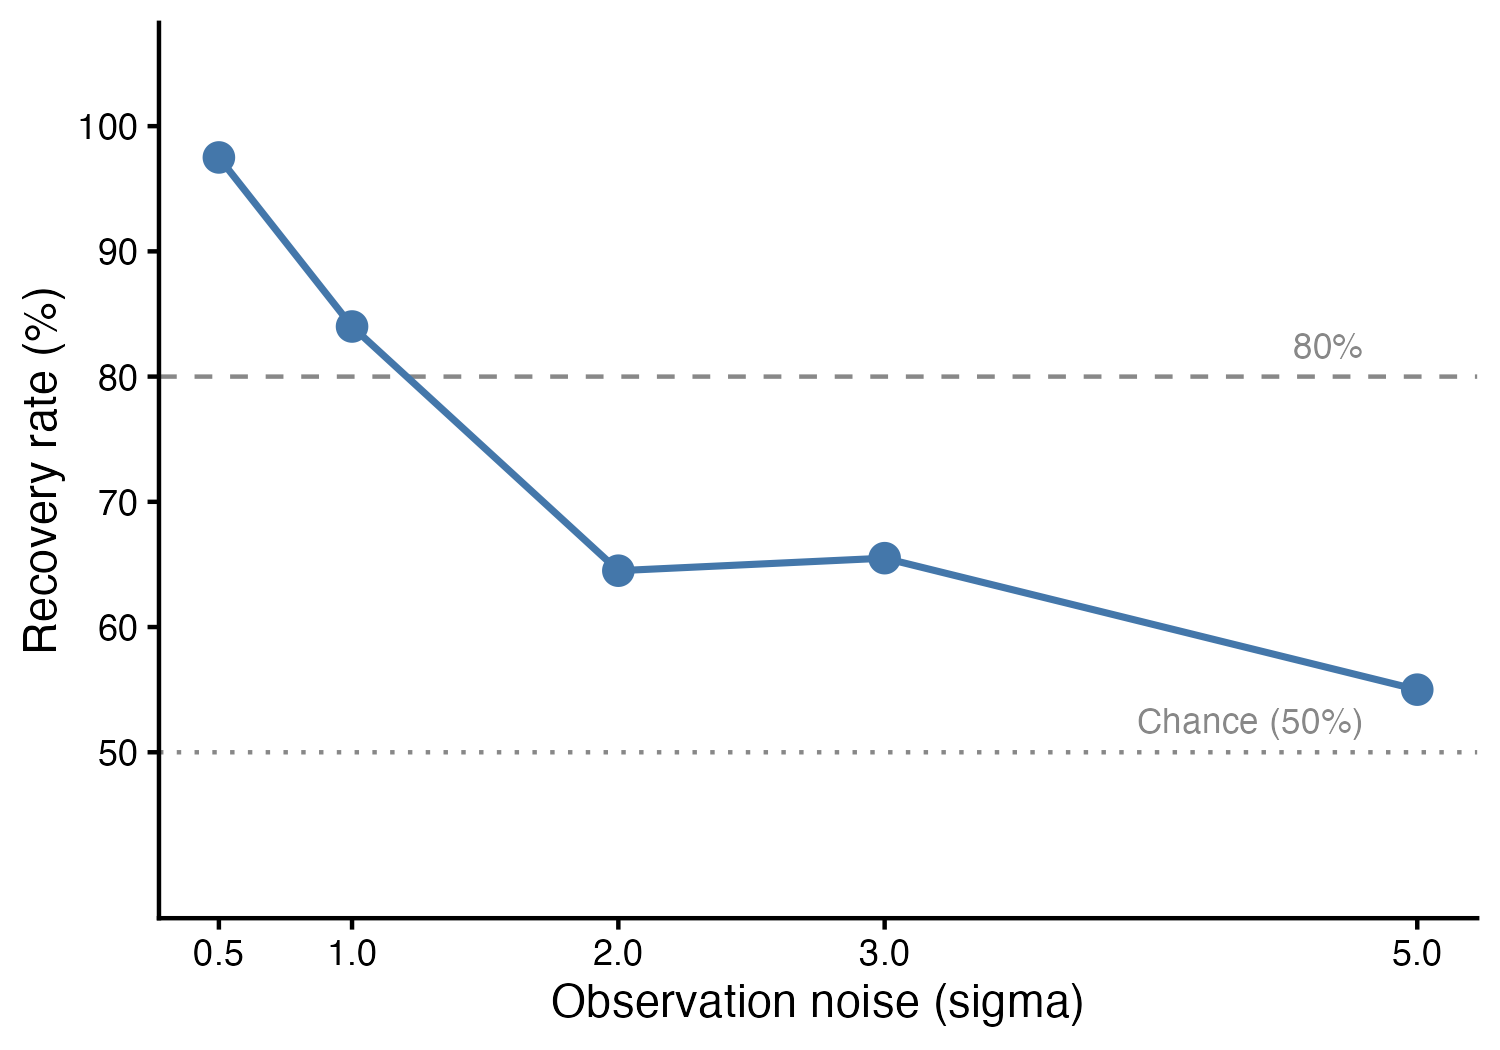
\includegraphics[width=0.65\linewidth]{Figures/figS4_model_recovery_noise.pdf}
\caption{Recovery rate as a function of observation noise $\sigma$, with $N = 30$ fixed. The dashed horizontal line marks 80\%; the dotted line marks chance (50\%). Recovery is near ceiling at $\sigma = 0.5$, drops sharply between $\sigma = 1.0$ and $\sigma = 2.0$, and approaches chance at $\sigma = 5.0$. The near-plateau at $\sigma = 2.0$ and $\sigma = 3.0$ is consistent with Monte Carlo variability (100 replications per model per noise level, SE $\approx 4\%$ at 65\%).}
\label{fig:s4_recovery}
\end{figure}

\subsection{Limitations and Implications}
\label{sec:s3_limits}

Three limitations apply. First, the SSE comparison uses a single reference prediction at the population mean rate ($\overline{S} = 0.30$), rather than fitting the model to each participant's individual data. This discards information about individual-level variation in $V_B$ and cannot capture how the distribution of $V_B$ values across participants differs between models. Per-participant maximum likelihood estimation would use this additional information and should yield higher recovery. Second, the generative bridge (Beta(3,\,7) individual differences, additive Gaussian noise) is the same in the generative and evaluative stages; the analysis does not test what happens when the bridge is misspecified. Third, only one $(N, \sigma)$ combination is explored in the main analysis; varying $N$ would produce a recovery curve analogous to the power curve in Section~5 of the main text.

Despite these simplifications, the exercise establishes a key qualitative finding: recovery around 80\% is achievable at $\sigma = 1.0$ and $N = 30$ under this simplified summary-level procedure. This is a precondition for a worthwhile experiment. Whether a full MLE analysis would achieve substantially higher recovery---and whether recovery degrades gracefully or sharply as noise increases---are empirical questions that the present demonstration does not answer, but which the companion code (\texttt{analysis/08\_model\_recovery.R}) can be extended to address.

Together with the power analysis in the main text, this section illustrates that \emph{detectability} and \emph{recoverability} are distinct inferential targets. A design can have adequate statistical power to detect a group-level deviation from the null while still supporting only modest model recovery under simplified comparison rules. Power analysis asks: given that the generating model is $M$, how often does a statistical test reject the null? Model recovery asks: given the observed data, does the correct model score better than the competitor? Both constraints bear on pre-data planning, and for studies designed to discriminate between models, pre-data planning ideally considers both. The present materials provide starting-point estimates for each.

Finally, the present simulations compare mechanistic consequences under representative parameterizations; they do not constitute complexity-penalized evidential adjudication between models with unequal flexibility. A formal complexity analysis would require computing marginal likelihoods (which in turn requires specifying a shared parameter prior), minimum description lengths, or penalized-likelihood scores such as BIC---tasks that go well beyond the scope of a tutorial demonstration. This limitation is flagged explicitly so that readers do not mistake the recovery exercise for a Bayes-factor or MDL comparison. The simulations demonstrate that the two models can be distinguished by a simple summary statistic under moderate noise; they do not demonstrate that one model is favored by a principled measure of relative evidential support.


\bibliographystyle{apalike}
\bibliography{references}

\end{document}
